\chapter{Results}\label{chapt:results}
% [\textit{ Report the results of the simulations. Validate your work, i.e. show that the computational model (\ref{chapt:model}) and the simulations you run (the DoE \ref{chapt:doe}) were able to obtain the goal of the project}]

With so much to talk in this report, everything can be summarised into a small picture - Figure~\ref{fig:the_complete_picture}

\section{Pros}
The model predicted most of the roads, which were predicted by the model without super-resolution. Apart from that, the model also predicted a lot of other small roads. On validating with the ground truth images, I found that this was a very good prediction. Figure~\ref{fig:run_merge_road_maps}

\begin{figure}[h!]
  \centering
  \begin{subfigure}{0.71\textwidth}
    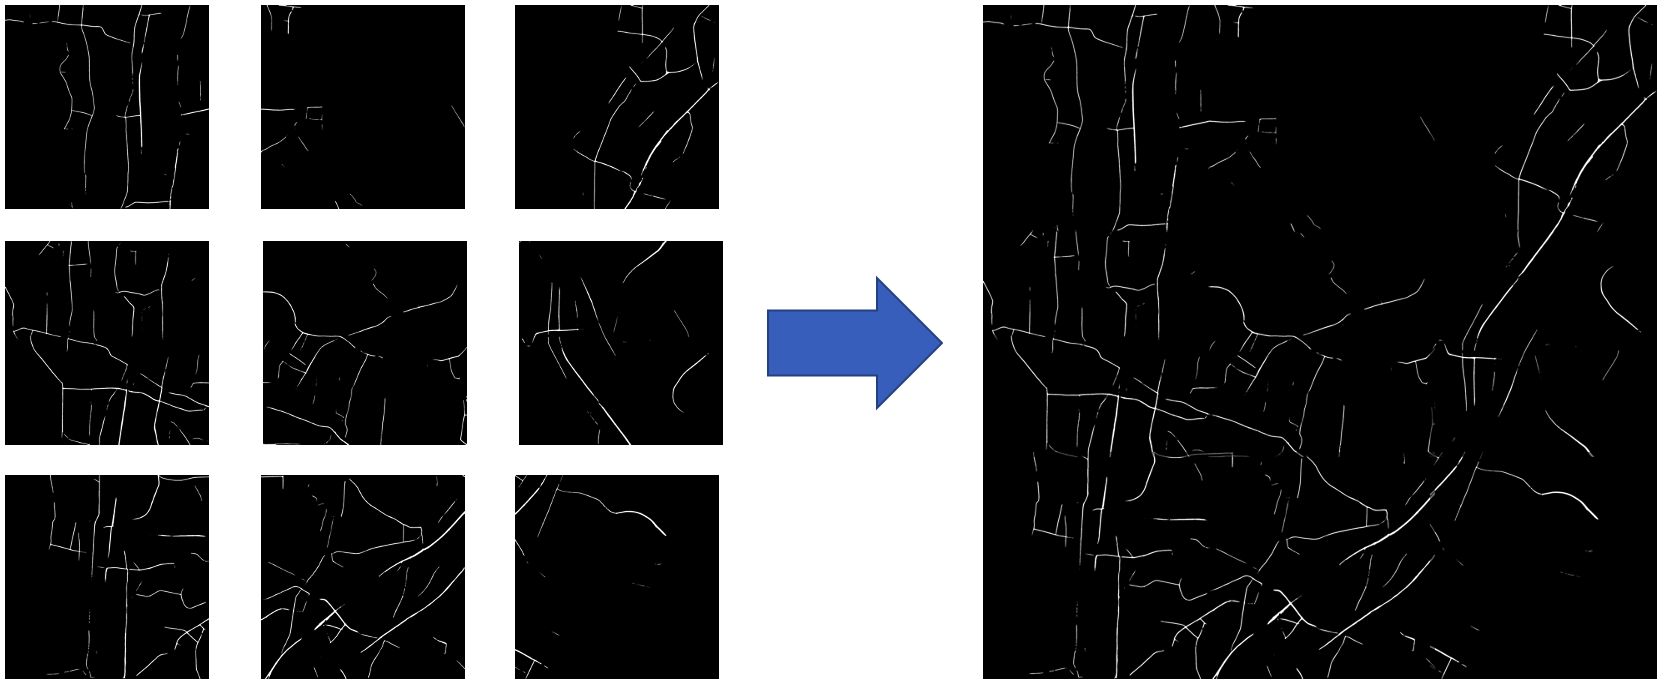
\includegraphics[width=\textwidth]{run_merge_roads}
    \caption{}
  \end{subfigure}~
  \begin{subfigure}{0.29\textwidth}
    \includegraphics[width=\textwidth]{sat_image_run}
    \caption{}
  \end{subfigure}
  \caption[Finding likeliness of roads by combining results from different models]{Merging roads as obtained by prediction from model.}
  \label{fig:run_merge_road_maps}
\end{figure}



\section{Cons}
One of the most noticeable drawbacks of using this model is the amount of time required to get the predictions. 

Another disadvantage is too much affected due to inaccuracies in the training dataset. If the road gets too thick, like, say, we took an image with a little higher resolution, and run the model; we see that our model has several discontinuities in between. This is mainly because of the noise which has effected the weights. This error can be reduced by training the model with more precise data. Another way to correct this error is to run the algorithm without super-resolution. This means we need to train the model again, this time without super-resolution.

% TODO: Add the image of without SR, use it as a con on the thick road.

Now that we have two predictions, one with super-resolution and without it, we merge them. First, we need to make them of the same resolutions. We do this by finding out the difference factor. Let us say the difference factor is x on each side; we split the lower resolution image pixels into x different pixels on both sides. Then we average the resultant images of the same resolution. For reference: look at Figure~\ref{fig:roads_in_confidence}

\begin{figure}[h!]
  \begin{subfigure}[b]{0.25\textwidth}
    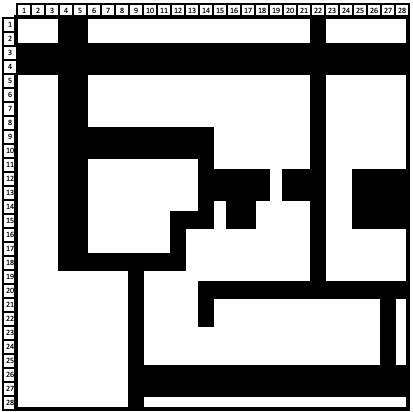
\includegraphics[width=\textwidth]{roads_with_SR}
    \caption{}
  \end{subfigure}~
  \begin{subfigure}[b]{0.15\textwidth}
    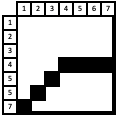
\includegraphics[width=\textwidth]{roads_without_SR}
    \caption{}
  \end{subfigure}~
  \begin{subfigure}[b]{0.25\textwidth}
    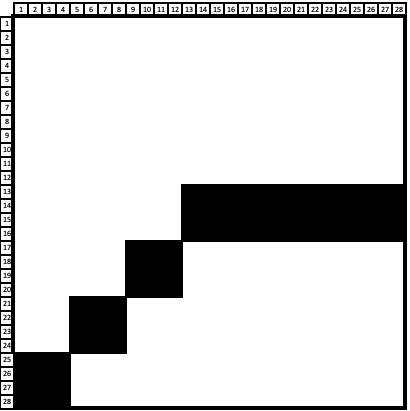
\includegraphics[width=\textwidth]{roads_without_SR_zoomed}
    \caption{}
  \end{subfigure}~
  \begin{subfigure}[b]{0.25\textwidth}
    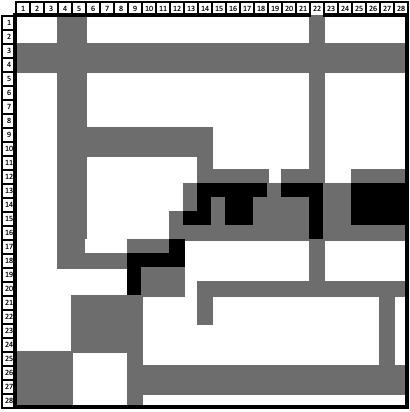
\includegraphics[width=\textwidth]{roads_with_confidence}
    \caption{}
  \end{subfigure}
  \caption[Finding likelihood of roads in predictions.]{Merging roads found with (a) Predictions with SR, (b) Predictions without SR. (c) Upscaling of (b) and (d) Final result by averaging (a) and (c). Black ones are definitely a road, Grey ones having 0.5 probablity of being a road and  least likely to find a road on the white pixel.}
  \label{fig:roads_in_confidence}
\end{figure}




\begin{sidewaysfigure}
  \centering
  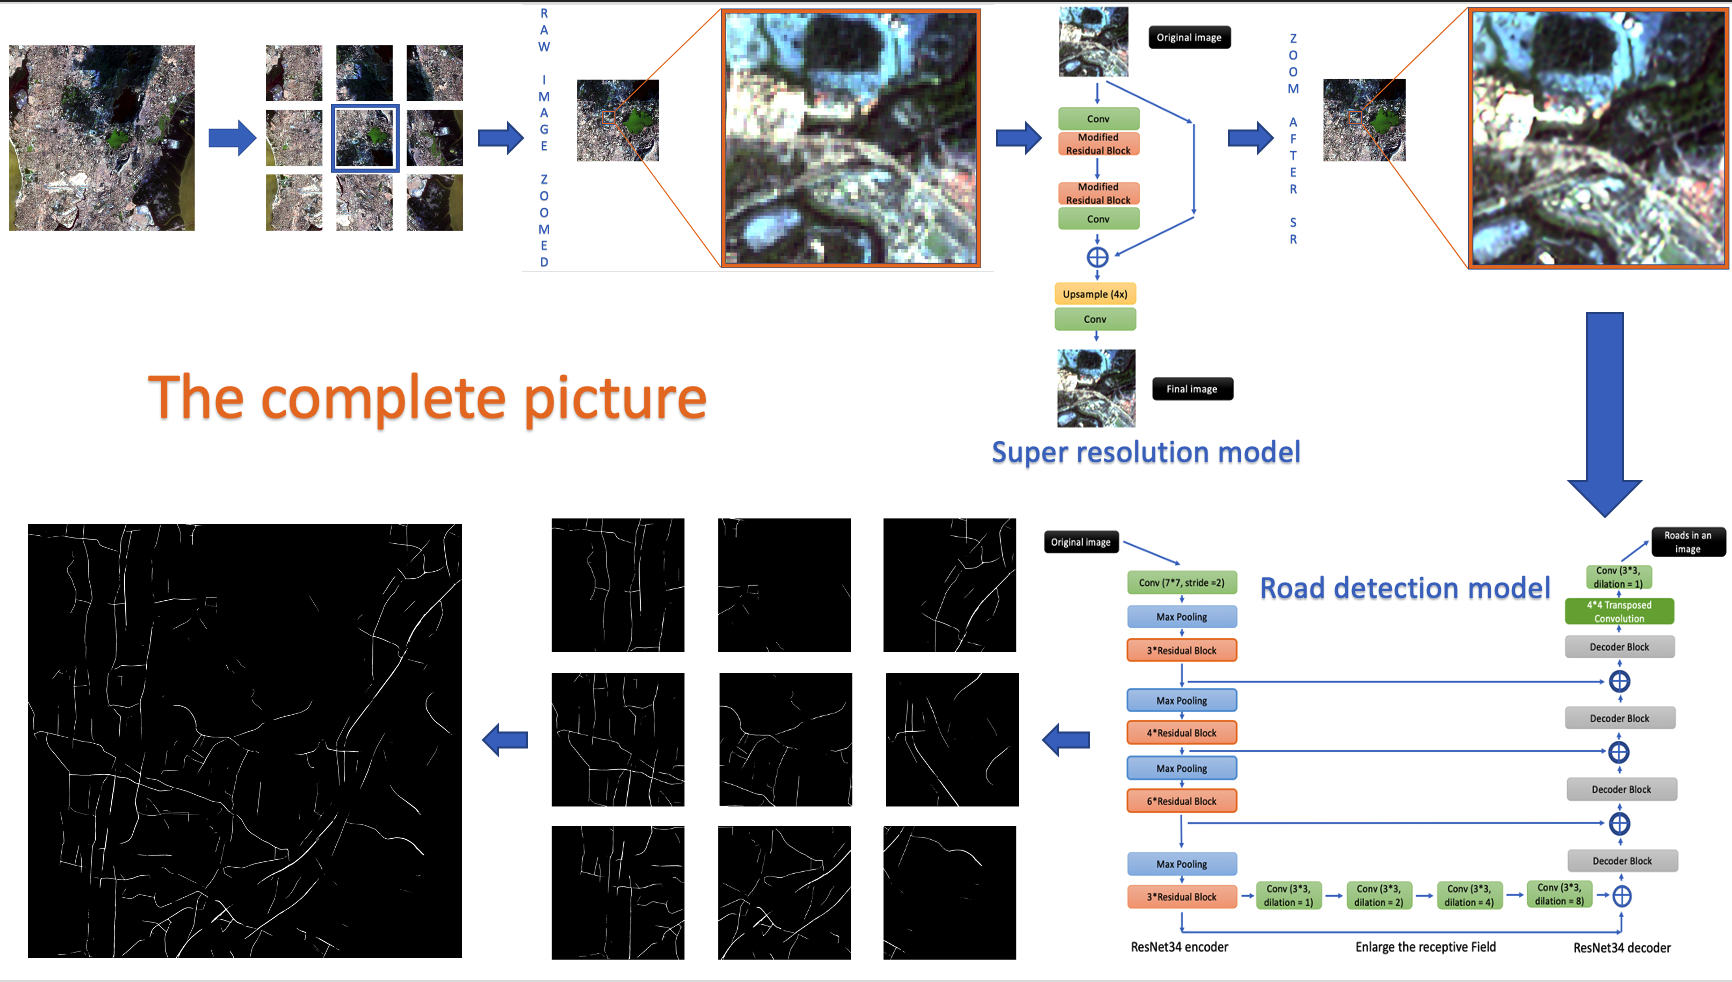
\includegraphics[width=\textheight]{the_complete_picture}
  \caption{A figure summarising the complete process into one}
  \label{fig:the_complete_picture}
\end{sidewaysfigure}

% \subsection{Test 2} ... as needed

\chapter{Conclusions}
\chapter{Scope of Improvements}
https://towardsdatascience.com/road-segmentation-727fb41c51af
\pagebreak
